\documentclass[11pt]{article}
\usepackage[utf8]{inputenc}
\usepackage{amsmath,amssymb}
\usepackage{graphicx}
\usepackage{hyperref}

\title{Sparse Attention for Long Documents}
\author{A. Researcher \and B. Student}
\date{\today}

\begin{document}
\maketitle

\begin{abstract}
We study sparse attention patterns for long documents and show that a simple
block-local scheme matches dense attention on three benchmarks.
\end{abstract}

\section{Introduction}
Transformers scale quadratically with sequence length~\cite{vaswani}. Prior work
reduces this cost with fixed patterns; see \url{https://example.org/survey} for a survey.

\section{Method}
Given queries $Q$, keys $K$ and values $V$, attention is
\begin{equation}
  \mathrm{Attn}(Q,K,V) = \mathrm{softmax}\left(\frac{QK^\top}{\sqrt{d}}\right)V.
  \label{eq:attn}
\end{equation}
We restrict \eqref{eq:attn} to blocks of size $b$.

\begin{figure}[t]
  \centering
  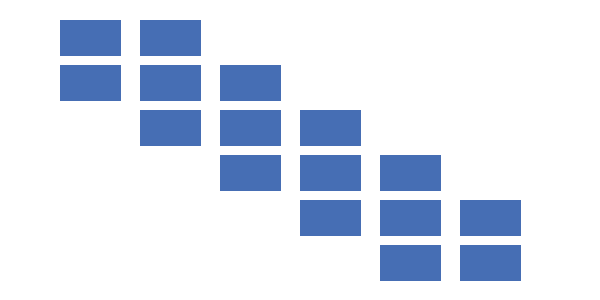
\includegraphics[width=0.8\textwidth]{blocks.png}
  \caption{Block-local attention pattern.}
  \label{fig:blocks}
\end{figure}

\section{Results}
Figure~\ref{fig:blocks} shows the pattern. Table~\ref{tab:res} lists the scores.

\begin{table}[h]
  \centering
  \begin{tabular}{lcc}
    \hline
    Model & Accuracy & Speed \\
    \hline
    Dense & 91.2 & 1.0 \\
    Sparse & 90.8 & 3.4 \\
    \hline
  \end{tabular}
  \caption{Results on the benchmark.}
  \label{tab:res}
\end{table}

\begin{thebibliography}{9}
\bibitem{vaswani} A. Vaswani et al. Attention is all you need. 2017.
\end{thebibliography}
\end{document}
